%% Beginning of file 'sample631.tex'
%%
%% Modified 2022 May  
%%
%% This is a sample manuscript marked up using the
%% AASTeX v6.31 LaTeX 2e macros.
%%
%% AASTeX is now based on Alexey Vikhlinin's emulateapj.cls 
%% (Copyright 2000-2015).  See the classfile for details.

\documentclass[preprint]{aastex631}

%% The default is a single spaced, 10 point font, single spaced article.
%% There are 5 other style options available via an optional argument. They
%% can be invoked like this:
%%
%% \documentclass[arguments]{aastex631}
%% 
%% where the layout options are:
%%
%%  twocolumn   : two text columns, 10 point font, single spaced article.
%%                This is the most compact and represent the final published
%%                derived PDF copy of the accepted manuscript from the publisher
%%  manuscript  : one text column, 12 point font, double spaced article.
%%  preprint    : one text column, 12 point font, single spaced article.  -> changed to 10pt
%%  preprint2   : two text columns, 12 point font, single spaced article.
%%  modern      : a stylish, single text column, 12 point font, article with
%% 		  wider left and right margins. This uses the Daniel
%% 		  Foreman-Mackey and David Hogg design.
%%  RNAAS       : Supresses an abstract. Originally for RNAAS manuscripts 
%%                but now that abstracts are required this is obsolete for
%%                AAS Journals. Authors might need it for other reasons. DO NOT
%%                use \begin{abstract} and \end{abstract} with this style.
%%
%% Note that you can submit to the AAS Journals in any of these 6 styles.
%%
%% There are other optional arguments one can invoke to allow other stylistic
%% actions. The available options are:
%%
%%   astrosymb    : Loads Astrosymb font and define \astrocommands. 
%%   tighten      : Makes baselineskip slightly smaller, only works with 
%%                  the twocolumn substyle.
%%   times        : uses times font instead of the default
%%   linenumbers  : turn on lineno package.
%%   trackchanges : required to see the revision mark up and print its output
%%   longauthor   : Do not use the more compressed footnote style (default) for 
%%                  the author/collaboration/affiliations. Instead print all
%%                  affiliation information after each name. Creates a much 
%%                  longer author list but may be desirable for short 
%%                  author papers.
%% twocolappendix : make 2 column appendix.
%%   anonymous    : Do not show the authors, affiliations and acknowledgments 
%%                  for dual anonymous review.
%%
%% these can be used in any combination, e.g.
%%
%% \documentclass[twocolumn,linenumbers,trackchanges]{aastex631}
%%
%% AASTeX v6.* now includes \hyperref support. While we have built in specific
%% defaults into the classfile you can manually override them with the
%% \hypersetup command. For example,
%%
%% \hypersetup{linkcolor=red,citecolor=green,filecolor=cyan,urlcolor=magenta}
%%
%% will change the color of the internal links to red, the links to the
%% bibliography to green, the file links to cyan, and the external links to
%% magenta. Additional information on \hyperref options can be found here:
%% https://www.tug.org/applications/hyperref/manual.html#x1-40003
%%
%% Note that in v6.3 "bookmarks" has been changed to "true" in hyperref
%% to improve the accessibility of the compiled pdf file.
%%
%% If you want to create your own macros, you can do so
%% using \newcommand. Your macros should appear before
%% the \begin{document} command.
%%

\usepackage{subfiles}
\newcommand{\vdag}{(v)^\dagger}
\newcommand\aastex{AAS\TeX}
\newcommand\latex{La\TeX}
\usepackage{times}

\begin{document}

\title{Lunar Farside Technosignature \& Transients Telescope (LFT3)}

\author[0000-0003-3197-2294]{David R. DeBoer}
\affiliation{Radio Astronomy Laboratory \\
University of California \\
Berkeley, CA, 94720 USA}
\author[0000-0002-0387-6476]{Karl F. Warnick}
\affiliation{ECEn Dept., Brigham Young University, Provo, UT, USA}



\begin{abstract}
Humanity is at a tipping point for a transition from earth-based observatories to space-based telescopes for radio astronomy. Cost-effective access to space means thousands of new RFI sources in orbit and a major degradation in the earth’s already challenging RF environment. It also makes possible a revolution in science access that is driving nations to send experiments to the lunar surface and orbit. The lunar farside offers a unique place and time to measure radiation from the Universe with essentially no radio frequency interference. We propose a UHF phased array telescope to be landed near the lunar antipode within 5 years to conduct initial baseline observations in the absence of RFI. The Lunar Farside Technosignatures \& Transients Telescope (LFT3) will search the farside sky for radio emissions from known and unknown sources and create a historical record of lunar radio observations from the current pristine silence to a more crowded environment as further instruments are deployed. LFT3 is a once-in-human-history opportunity to record signals in a fully quiet environment. 

\end{abstract}

\section{Introduction} 
\label{sec:intro}
\subfile{introduction}

\section{Science Case}
\label{sec:science}
\subfile{science}

\section{Observing Within The Terrestrial RF Environment}
\label{sec:rfenv}
\subfile{terrestrial_rf}

\section{Payload Overview}
\label{sec:payload}
%\subfile{payload}

The science payload includes a mid-band phased array operating from 300--900 MHz, a wide band and high band antenna (600-1800 MHz), an ``FM'' band antenna (80--110 MHz), and a low band antenna (1--50 MHz). 

The mid-band array covers the bulk of the lander top surface with 48 dual polarizatio wideband antenna elements. The array forms a fan of beams on the sky designed to cover most of the lunar sky over time (Fig.\ \ref{fig:midband_beam_maps}). Formed beam output signals are downconverted and sampled in a  50 MHz subband that is tuned scanned repeatedly across the array operating bandwidth. 

\begin{figure}
	\centering
	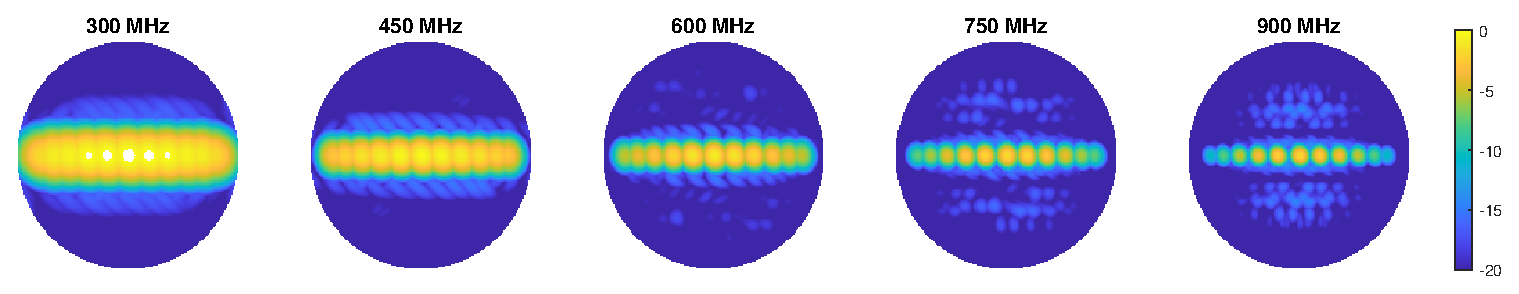
\includegraphics[width=\linewidth]{figures/midband_array_28cm_3dBSLL_beams_max.eps}
	\caption{Midband array formed beams over frequency. Scale is aperture efficiency in dB relative to a 3 meter diameter area. Beams are centered within 11 equal intervals over a 120 degree field of view.}
	\label{fig:midband_beam_maps}
\end{figure}

\begin{figure}
	\centering
	\includegraphics[width=\linewidth]{\begin{figure}
	\centering
	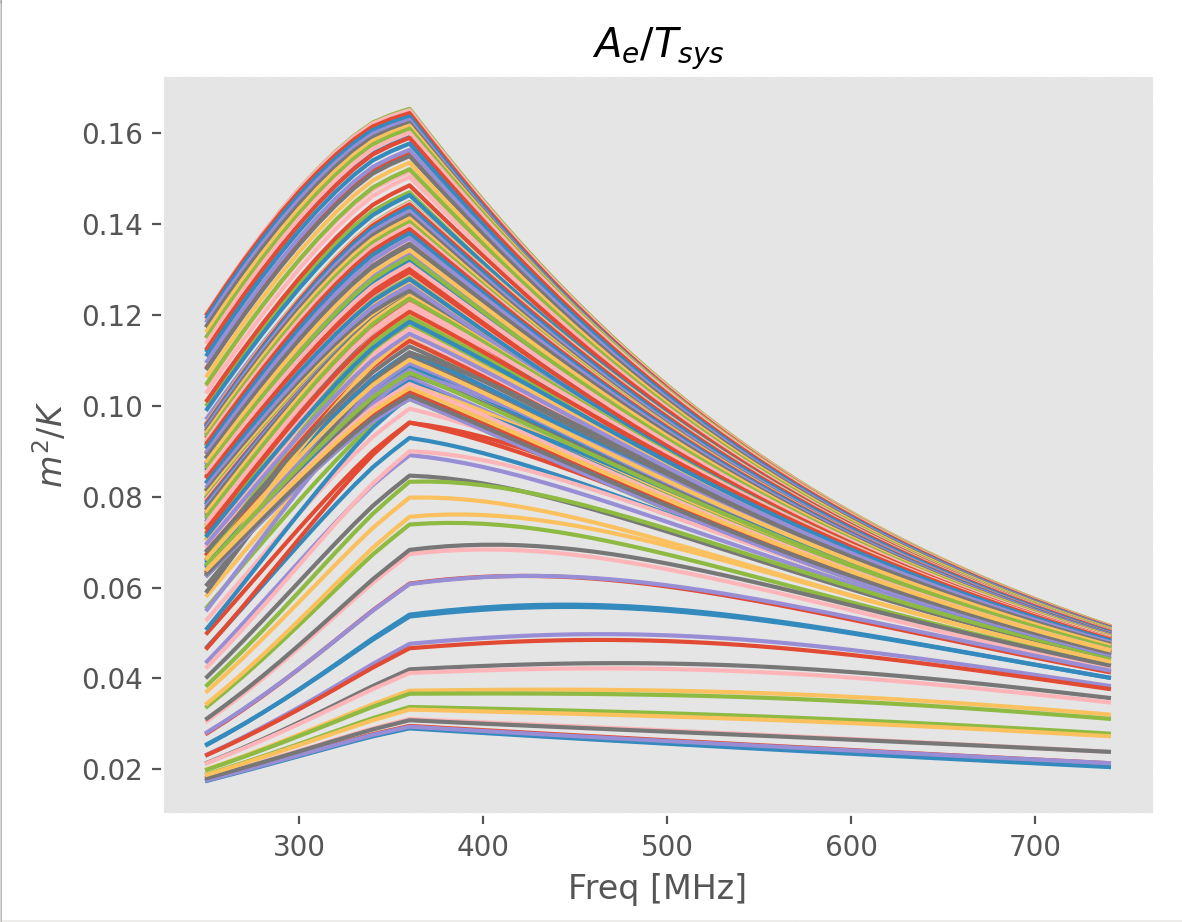
\includegraphics[width=\linewidth]{figures/sensitivity_early_est.png}
	\caption{Early estimates of sensitivity}
\end{figure}

\section{Operations Overview}
\label{sec:operations}
%\subfile{operations}

%\appendix
%\section{Appendix information}


\bibliography{bibs}{}
\bibliographystyle{aasjournal}

%% This command is needed to show the entire author+affiliation list when
%% the collaboration and author truncation commands are used.  It has to
%% go at the end of the manuscript.
%\allauthors

%% Include this line if you are using the \added, \replaced, \deleted
%% commands to see a summary list of all changes at the end of the article.
%\listofchanges

\end{document}

